%% Journal of Science and Medicine in Sport — Original Research (anonymised manuscript)
%% Built by bygg_jsams.py from the frozen ../manus/main.tex. Do not edit by hand.
\documentclass[12pt,a4paper]{article}

\usepackage[utf8]{inputenc}
\usepackage[T1]{fontenc}
\usepackage{times}
\usepackage[margin=2.5cm]{geometry}
\usepackage{setspace}
\doublespacing

\usepackage{graphicx}
\graphicspath{{../figures/}}
\usepackage{float}
\usepackage{placeins}
\usepackage{amsmath,amssymb}
\usepackage{booktabs}
\usepackage{caption}
\usepackage{enumitem}
\usepackage[colorlinks=true,linkcolor=blue,citecolor=blue,urlcolor=blue]{hyperref}
\usepackage[numbers,sort&compress]{natbib}
\usepackage{lineno}
\linenumbers

\begin{document}

\begin{center}
{\LARGE\bfseries Does starting age predict who stays? Competition debut and long-term participation in youth track and field\par}
\vspace{0.5em}
{\normalsize Anonymised manuscript --- Original Research\par}
\end{center}

\section*{Abstract}

\noindent\textbf{Objectives:} To test whether age at first registered competition predicts long-term participation, and whether entry history adds information beyond current engagement.

\noindent\textbf{Design:} Population-based registry cohort study.

\noindent\textbf{Methods:} All athletes born 2001--2005 with a first registered competition at ages 10--16 (n = 17\,496; 50\,\% female) were followed in the Norwegian Athletics Federation's registry to October 2026. The outcome was senior activity (at least two results in a season at age 20 or older). Debut age was modelled categorically and linearly by logistic regression adjusted for sex, cohort and club size; persistence was compared at equal career length; a landmark analysis of athletes competing at 17 added current competition volume.

\noindent\textbf{Results:} 546 (3.1\,\%) became active seniors. Conversion was U-shaped in debut age (non-linearity p $<$ 0.001): relative to debut at 10 (3.8\,\%), adjusted odds were lowest for debuts at 11--14 (odds ratio 0.53--0.75) and equal by 15, with a null linear trend (odds ratio 0.99 per year, 95\,\% confidence interval [CI] 0.94--1.04). At equal career length, later starters persisted less: 20.4\,\% of those debuting at 10 still competed four or more years later, against 4.5--6.6\,\% for debuts at 14--16 (odds ratio 0.70 per year, 95\,\% CI 0.68--0.72). At the age-17 landmark, earlier debut appeared advantageous (odds ratio 0.85 per year, 95\,\% CI 0.80--0.90) but not after adjusting for current volume (odds ratio 0.99, 95\,\% CI 0.92--1.05).

\noindent\textbf{Conclusions:} Early competitive entry did not undermine retention: per year of career, early entrants persisted longest. Among older adolescents, current engagement predicted retention better than entry history.

\vspace{0.5em}
\noindent\textbf{Keywords:} Athletes$^\dagger$; Adolescent$^\dagger$; Child$^\dagger$; Registries$^\dagger$; Cohort studies$^\dagger$; attrition

\noindent{\footnotesize $^\dagger$Medical Subject Headings (MeSH) term.}

\newpage
\section{Introduction}

When should children enter competitive sport? The question sits at the centre of the early-specialisation debate, and the two main positions make opposite predictions about participation. One line of argument, prominent in consensus statements, cautions that intensive training and competition at young ages risk overuse injury and burnout, the latter defined there as ceasing to participate in a previously enjoyable activity \cite{difiori2014}; read onto entry timing, later entry should then protect retention. The opposite prediction comes from the retention literature itself: in a large prospective dropout study among 1\,762 Dutch football players, those who dropped out had \emph{started organised football later} than those who stayed, and the authors suggested that attracting children from about age six might reduce dropout \cite{vanyperen2021} --- though its exposure, joining organised football, is not the same construct as the registered-competition debut studied here, a gap we keep explicit throughout. Direct tests are scarce. In one of the few studies to measure both, markers of early specialisation were not positively related to burnout or dropout among age-group swimmers \cite{larson2019}; a systematic review of youth sport dropout identified lack of enjoyment, perceived competence, social pressures, competing priorities and physical factors, not starting age \cite{crane2015}, and in a Norwegian survey of dropouts' own reasons the most common were schoolwork, lacking skills and friends who quit, with cost and parental discouragement socially patterned \cite{espedalen2022}; and the retrospective expertise literature --- which finds that adult world-class athletes started their main sport later than national-class peers \cite{barth2022}, and that youth and adult top performers are largely different people \cite{gullich2025} --- samples on success and therefore cannot speak to population-level retention. No study has followed a complete national entry population of an individual sport and asked what age at entry implies for who is still competing a decade later.

The Norwegian athletics registry permits exactly that design. Every sanctioned result in Norway is registered, the registry holds results electronically from 2011, and competition begins at age 10. For athletes born in 2001 or later, the competitive career is therefore observed from its first registered result, for everyone who ever entered, not only for those who later succeeded --- although coverage in 2011, the first electronic season, is thinner than in later years. Three other studies of the same registry frame the present one. Relative-age selection was found to be fully established at the entry stage and stable thereafter, locating the system's selection pressure at the point of entry rather than in adolescent talent identification \cite{guttormsen2026rae}. A 14-year cohort study found that competition volume at ages 13--14 predicted senior retention somewhat better than performance did, and that exit is preceded by behavioural withdrawal (unpublished data). A further study of performance trajectories in the registry found that progression predicts retention beyond volume --- but that, here too, the \emph{recent} window dominates the earlier one (unpublished data). Against that background, entry age is the natural next exposure: it is the first \emph{registered} behavioural fact the registry holds about an athlete --- prior training and other sports are invisible to it.

We pre-specified three questions. \textbf{H1:} among all athletes whose first registered competition fell at ages 10--16, is debut age associated with being active as a senior? Read onto this entry-timing margin, the two positions above suggest opposite directions, so H1 is two-sided, a U-shape is plausible, and the categorical contrast is the primary display. \textbf{H2:} once started, do later debutants exit faster, as the football findings suggest \cite{vanyperen2021}? \textbf{H3:} among athletes still active at age 17, does entry history add anything beyond current engagement --- or does the registry repeat its now-familiar lesson that current behaviour dominates history (unpublished data)? Interpretation rules were fixed in advance: the exposure is \emph{competition debut}, not the start of sport participation or training, and selection into late debut (already-interested adolescents choosing athletics) is expected and addressed in the design and interpretation. The analysis plan was committed to version control before any exposure--outcome model was estimated; the study was not externally preregistered.

% ════════════════════════════════════════════════════════════
\section{Methods}

\subsection{Data source and design}

The Norwegian Athletics Federation's results database registers every sanctioned competition result in Norway and Norwegian athletes' results abroad. We used a frozen extract of 29 October 2026 (results dated on or before that day). Only participation fields were extracted --- athlete, date, meet, club, approval status; no performance data of any kind were used at any age, in keeping with the purpose of the Norwegian children's sport regulations. Age is calendar-year age (competition year minus birth year), the basis of Norwegian age classes. Reporting follows STROBE \cite{vonelm2007}.

\subsection{Sample}

All athletes born 2001--2008 entered the extraction (n = 33\,666, with 675\,707 result rows; 1\,526 non-approved rows and 116 rows below age 10 were excluded). The 28\,339 athletes with an approved result at age 10 or older constitute the debutant population; 865 without registered sex (predominantly brief, early participants) were excluded, and of the remaining 27\,474, 731 (2.7\,\%) whose debut fell at age 17 or later were set aside (those born 2001--2005 with debut at 17--19 form a sensitivity category). Of the remaining 26\,743 debutants, the primary sample comprises the 17\,496 born 2001--2005 with debut at ages 10--16 --- cohorts whose follow-up extends past age 20 for everyone --- of whom 50.1\,\% were female and 546 (3.1\,\%) met the senior-activity outcome; the other 9\,247, born 2006--2008, contribute to descriptive analyses of entry patterns only. Because non-approved rows and sub-age-10 rows were excluded before debut assignment, 49 athletes in the primary sample (0.3\,\%) had earlier excluded rows, which would change the debut age of 33 of them. The full sample flow is given in Supplementary Table S1.

\subsection{Exposure, outcomes, and covariates}

The exposure is \emph{debut age}: calendar-year age at the athlete's first approved registered result (10--16), treated categorically (reference: debut at 10) and as a linear trend. The primary outcome, identical to the earlier studies of this registry (unpublished data), is \emph{active senior}: at least two approved results in the same calendar year at age 20 or older. Secondary outcomes were at least one result at age $\geq$20, activity at age $\geq$17, and retention $k$ years after debut ($k$ = 1--5), defined as at least one approved result in the calendar year debut + $k$ (point prevalence), computed with per-$k$ denominators over athlete-years fully observable by 2025. Because the senior outcome is defined at a fixed age, later entrants have fewer years to cover before it; we therefore added an outcome measured at equal career length: at least two competition days in a single season four or more years after the debut season (five and six years as sensitivity analyses), each among athletes for whom that season was fully observable by 2025. Covariates were sex, birth cohort, and baseline club (modal club in the debut season) with the logarithm of a club-size proxy (study athletes per club); debut-season competition days and a COVID-19 flag for debuts in 2020--2021 were used in robustness analyses, and birth quarter (where an exact birth date existed) is described but enters no reported model. Covariate sets per hypothesis: the H1 and equal-career-length models adjust for sex, cohort, and club size, and robustness variants of the H1 trend exclude COVID-era debuts or add debut-season days; the landmark models use sex and cohort, with current competition days added in the second specification. Region, specified in the analysis plan, could not be adjusted for: the registry records the competition district for under 1\,\% of meets. Full coefficient tables are available with the analysis code.

\subsection{Statistical analysis}

H1 was estimated by logistic regression in the primary sample, with debut age categorical and linear, adjusted for sex, cohort, and club size, with club-clustered standard errors as a sensitivity. H2 was addressed on both clocks without imposing a survival model. On the \emph{duration} clock --- the comparison that aligns athletes at the same career stage --- we report the proportion still competing $k$ years after their own debut, by debut age, and model the equal-career-length outcome with the H1 covariates. On the \emph{age} clock we report, for the cohorts born 2001--2004 (followed to age 21 for everyone), the share of each debut group with a registered result at that age or later. The analysis plan specified an age-scale Cox model with delayed entry at debut and delayed-entry Kaplan--Meier curves \cite{korn1997}; both were replaced, because exit risk depends on time since debut: the proportional-hazards assumption then fails by construction, and the delayed-entry product-limit estimator multiplies the first-season exits of different entry ages into a single curve that no cohort experiences. Age equals debut age plus career duration, so neither clock isolates an effect of entry age, and both are reported descriptively. The 2026 season is observed to 29 October, which slightly shortens the senior window of the youngest cohort --- the cohort covariate and the cohort-split robustness address this. H3 was a landmark analysis \cite{anderson1983} among athletes with at least one approved result \emph{in the age-17 season itself} --- not merely any result at age 17 or later, which would let future senior activity qualify athletes into the landmark and thereby condition on the outcome's own future. Senior activity was regressed on debut age with sex and cohort, with and without current engagement (competition days at ages 16--17, standardised); the landmark sits at the end of the age-17 season, all predictors are measured by then, and the outcome window begins at age 20. Sex-specific conversion and a sex $\times$ debut-age interaction were also examined. Pre-specified robustness analyses excluded COVID-19 debuts, varied the outcome, added debut-season volume, split the cohorts (2001--2003 vs.\ 2004--2005), and included debut at 17--19 as a category. After the plan was committed we added a likelihood-ratio test comparing the categorical and linear codings, analyses excluding the 2001 cohort, whose debut-at-10 season (2011) has the thinnest coverage, analyses including athletes without registered sex as a separate category, and the COVID-19 exclusion, the COVID-19 flag and the cohort split applied to the categorical coding (the pre-specified versions concern the linear trend). The pre-specified debut age $\times$ birth-quarter interaction is not reported: exact birth dates exist for 98.5\,\% of the seniors but 51.9\,\% of the other athletes, and coverage rises steeply with debut age (Table~\ref{tab:char}), so the subsample is selected on both outcome and exposure. Analyses used Python 3.13.7 with pandas 2.3.3, numpy 2.4.1 and statsmodels 0.14.6.

\subsection{Ethics and transparency}

The data are competition results registered by the Norwegian Athletics Federation: results from age 13 are publicly listed, while records for the 10--12 age classes are registered but not publicly released by the federation, and for those ages only participation itself (whether and when an athlete competed) was used. No individual is identified and no performance data were used. As for the earlier studies of the same registry, the study is not medical or health research as defined by Norway's Health Research Act (Helseforskningsloven \S\S~2 and 4), so approval by a Regional Committee for Medical and Health Research Ethics was not required, and Sikt (the Norwegian Agency for Shared Services in Education and Research) confirmed that the use of the data raises no data-protection concerns. No participants were contacted or recruited, and informed consent was not required. The analysis plan, hypotheses, estimands, and interpretation rules were committed to version control before estimation; athlete-level files are regenerable from the registry.

% ════════════════════════════════════════════════════════════
\section{Results}

\subsection{Who debuts when}

Debut at 10, the first eligible age, was the single most common entry point, with a share rising from 32.6\,\% of debutants born 2001 to 43.9\,\% of those born 2008 --- a rise exaggerated at both ends, since the 2001 cohort's debut-at-10 season was 2011, the first and thinnest electronic season, and the 2008 cohort lost almost half of its debuts at 12 in the COVID-disrupted 2020 season (9.3\,\% debuted at 12, against 17.1--17.5\,\% in the two preceding cohorts). Late entry remained substantial: roughly one debutant in six entered at 14 or later (Figure~\ref{fig:cohort}). Table~\ref{tab:char} describes the three debut groups. Late debutants were more often male (female share 52.2\,\% for debut at 10--11 against 42.0\,\% for 14--16). The typical debut was brief in every group: the median debutant competed on a single day in the debut season, and median career length was two seasons for debut at 10--11 and one season otherwise. Entry intensity was thus flat across debut ages --- debut age is not a proxy for dose at entry. Exact birth dates --- needed for birth-quarter analyses --- existed for 38.6\,\% of early, 63.8\,\% of mid, and 88.5\,\% of late debutants, the registry's known pattern of missingness concentrating among brief early participants \cite{guttormsen2026rae}; among those with known dates, the fourth quarter was underrepresented at every debut age (Q1 25--31\,\% against Q4 19--22\,\%).

\begin{table}[H]
\centering
\caption{Characteristics of the primary sample (born 2001--2005, debut at ages 10--16), by debut group.}
\label{tab:char}
\small
\begin{tabular}{lccc}
\toprule
Characteristic & Debut 10--11 & Debut 12--13 & Debut 14--16 \\
\midrule
n & 10\,242 & 4\,220 & 3\,034 \\
Female, \% & 52.2 & 50.8 & 42.0 \\
Exact birth date available, \% & 38.6 & 63.8 & 88.5 \\
Born Q1, \% of those with birth date & 29.2 & 26.1 & 27.1 \\
Born Q4, \% of those with birth date & 19.9 & 21.9 & 19.8 \\
Competition days in debut season, median (IQR) & 1 (1--3) & 1 (1--3) & 1 (1--2) \\
Career length, seasons, median (IQR) & 2 (1--4) & 1 (1--3) & 1 (1--2) \\
Debut season 2020--2021, \% & 0.0 & 0.0 & 6.3 \\
\bottomrule
\end{tabular}

\vspace{0.3em}
\parbox{0.92\textwidth}{\footnotesize By construction, cohorts born 2001--2005 could only experience a 2020--2021 debut at ages 15 and 16. Abbreviations: IQR, interquartile range; Q1 and Q4, first and fourth quarter of the birth year.}
\end{table}

\begin{figure}[H]
\centering
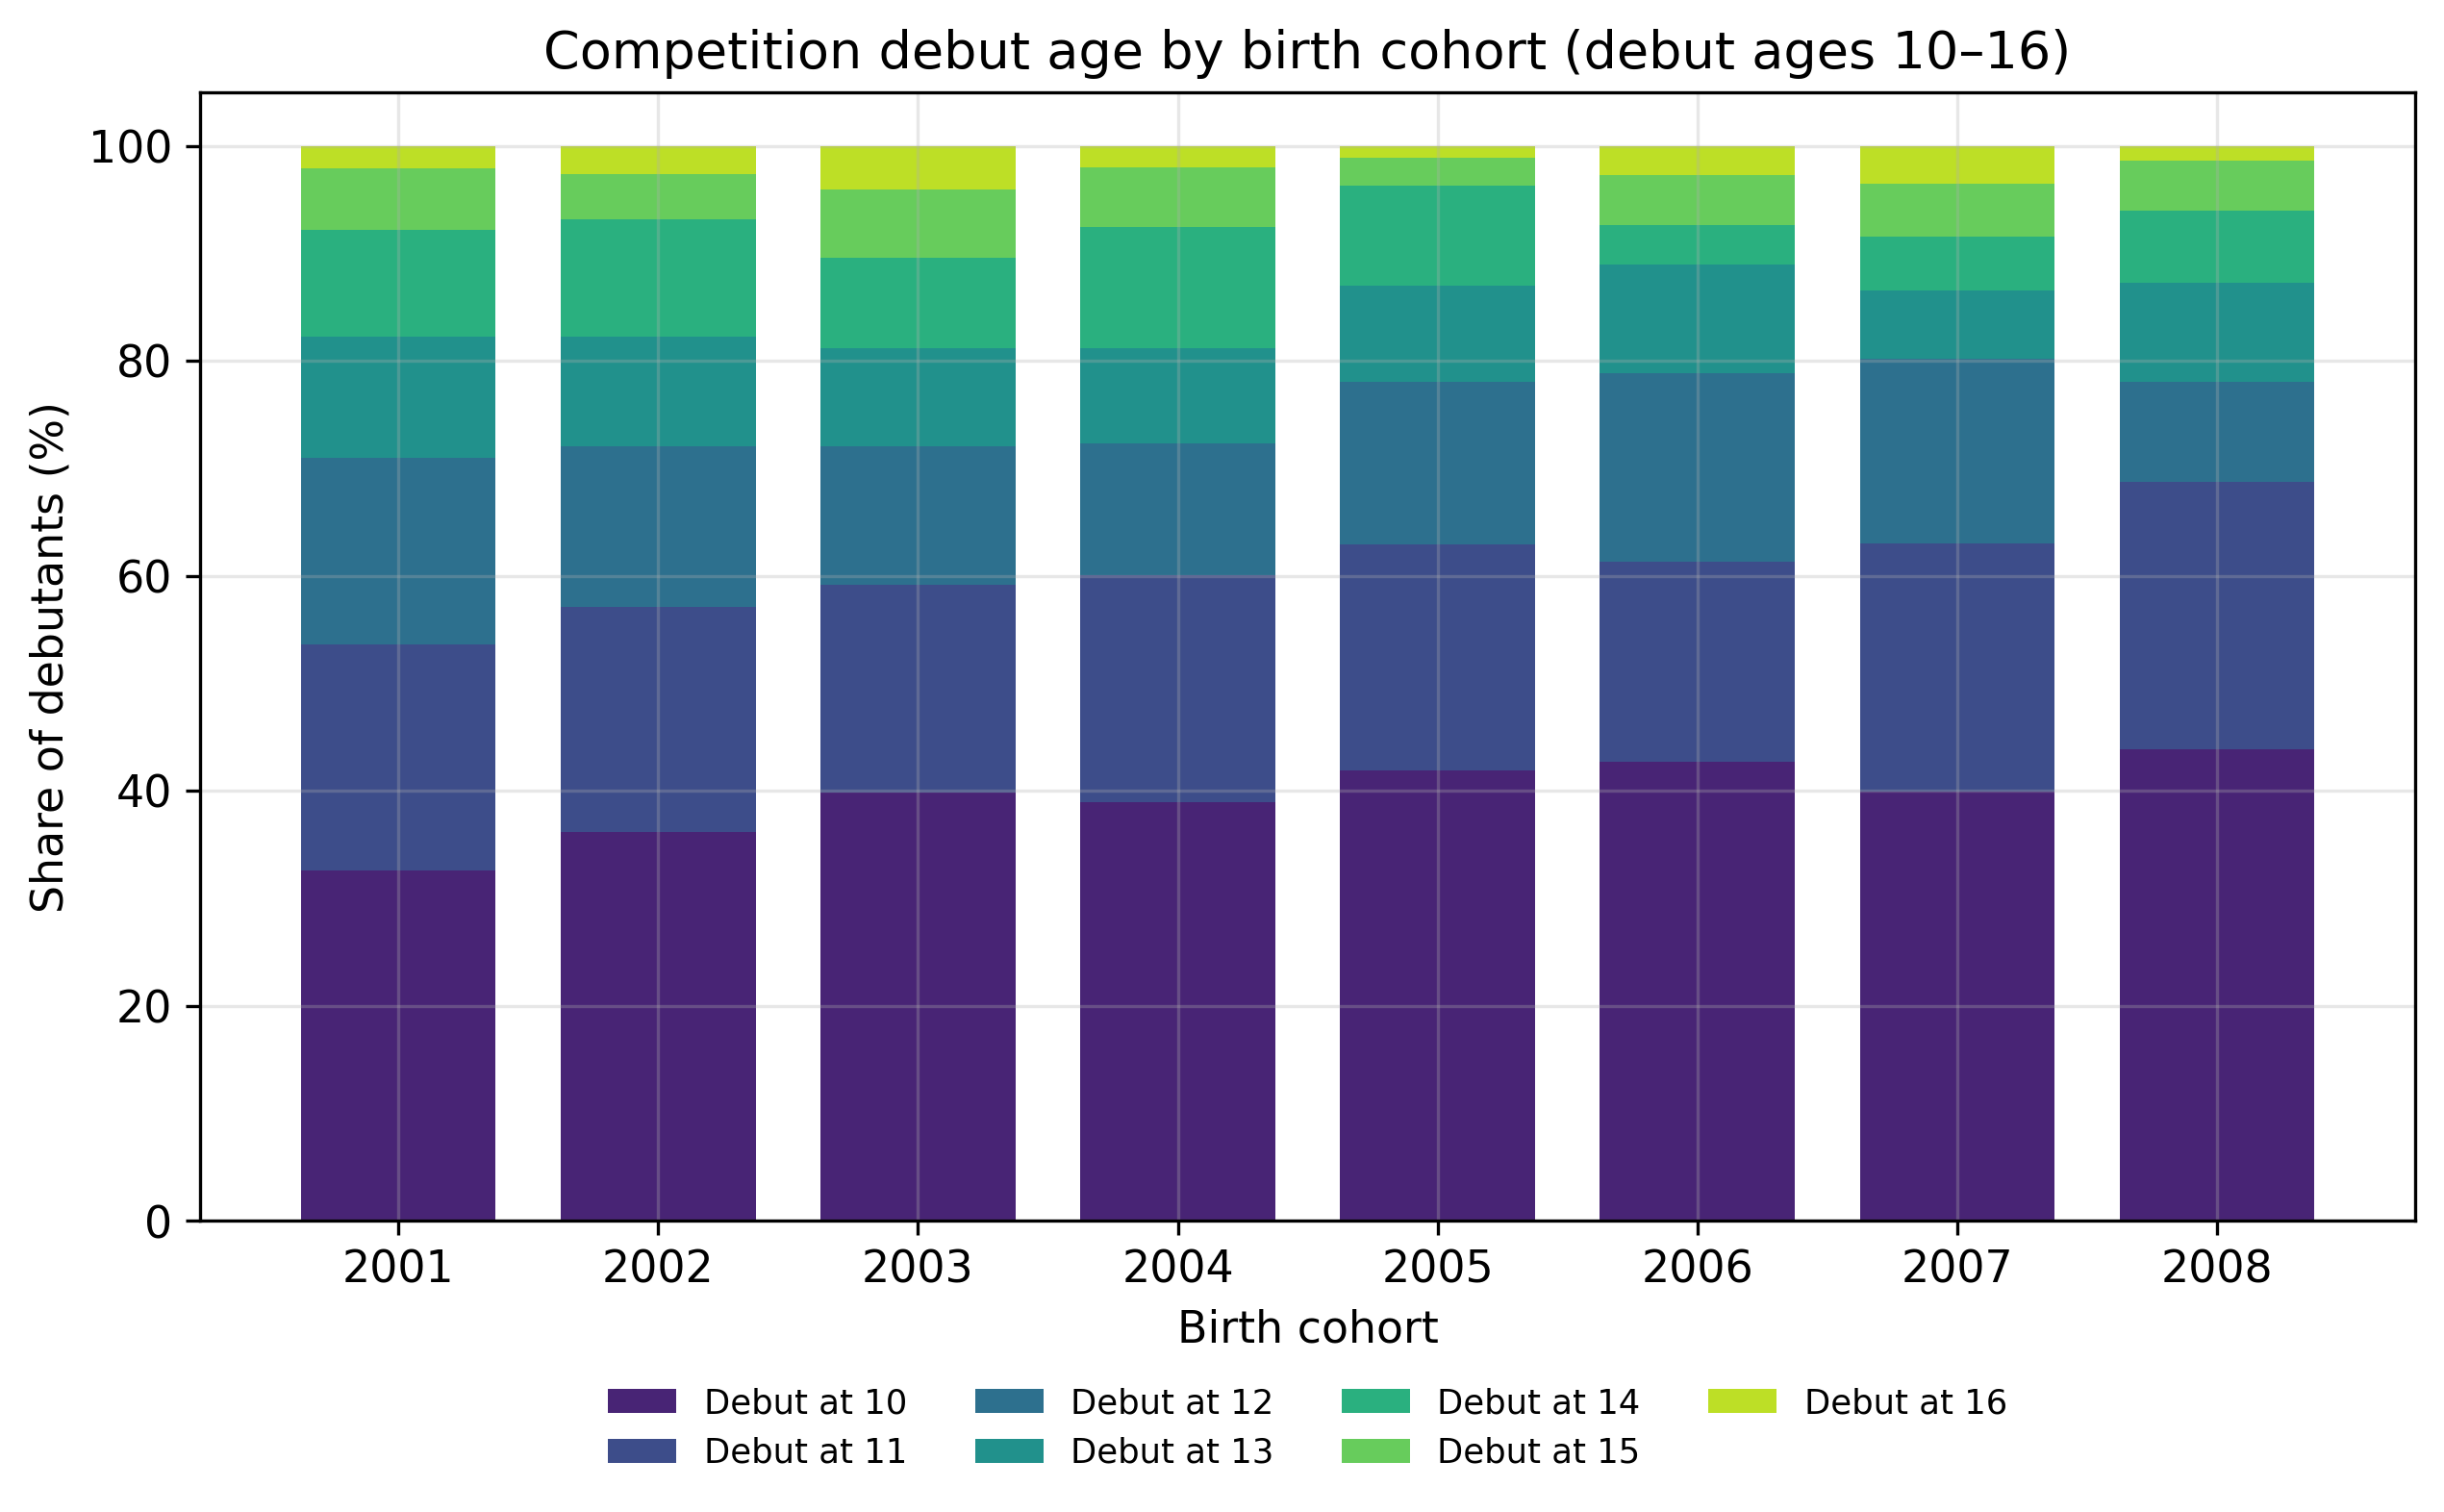
\includegraphics[width=0.85\textwidth]{fig1_debut_age_by_cohort.png}
\caption{Competition debut age by birth cohort (all debutants born 2001--2008, debut ages 10--16).}
\label{fig:cohort}
\end{figure}

\subsection{Senior conversion is U-shaped in debut age (H1)}

Of the 17\,496 debutants, 546 (3.1\,\%) were active as seniors. Conversion was not monotone in debut age (Figure~\ref{fig:ushape}): it was 3.8\,\% for debut at 10 (253/6\,626), fell to 2.4\,\% at 11, 2.1\,\% at 12, 2.9\,\% at 13 and 2.4\,\% at 14, and rose to 3.9\,\% at 15 and 6.6\,\% at 16 (28/424). A likelihood-ratio test rejected the linear coding in favour of the categorical one (LR = 43.2, df = 5, p = 3.3 $\times$ 10$^{-8}$): the association is non-linear. Adjusted for sex, cohort, and club size (Table~\ref{tab:h1}), debuts at 11, 12 and 14 had significantly lower odds than debut at 10 (OR 0.53--0.63), debut at 13 directionally lower odds (OR 0.75, 95\,\% CI 0.55--1.02), debut at 15 the same odds (OR 1.00), and debut at 16 higher odds (OR 1.73, 95\,\% CI 1.15--2.59, resting on 28 events). The linear trend across 10--16 was correspondingly null (OR 0.99 per year, 95\,\% CI 0.94--1.04) --- a flat average concealing a U. The elevation at 16, however, rests on debuts that fell in the COVID-19 seasons. All 107 debut-16 athletes born 2004--2005 debuted in 2020 or 2021, and 10.3\,\% of them became active seniors, against 5.4\,\% of the other 317 debut-16 athletes. Excluding 2020--2021 debuts, the debut-16 odds ratio was 1.32 (95\,\% CI 0.79--2.19), and with a COVID-19 flag in the model 1.38 (95\,\% CI 0.86--2.19), while the odds at 11--14 were unchanged (OR 0.53--0.75) and the association remained non-linear (LR = 30.5, df = 5, p = 1.2 $\times$ 10$^{-5}$; Supplementary Table S5). Because the outcome is defined at a fixed age, these rates compare entrants who had between four (debut at 16) and ten (debut at 10) seasons to cover before the outcome window; Section 3.3 measures persistence at equal career length. Conversion was higher for boys than girls at every debut age (4.3 vs.\ 3.4\,\% at debut 10; 7.1 vs.\ 5.7\,\% at debut 16; Supplementary Table S2), and the late-entry channel is male-tilted in composition (42.0\,\% female at debut 14--16); the sex $\times$ debut-age interaction was directionally negative but not significant (OR 0.92 per year, 95\,\% CI 0.82--1.02), and the raw conversion rates show the same U in both sexes (Supplementary Table S2).

\begin{table}[H]
\centering
\caption{Senior activity (age $\geq$20) and competing at equal career length, by debut age (n = 17\,496; 546 senior events, 2\,312 equal-career-length events). \% = raw proportion; odds ratios relative to debut at age 10, adjusted for sex, birth cohort, and club size. Competing $\geq$4 years after debut: at least two competition days in a single season four or more years after the debut season. A likelihood-ratio test favours the categorical over the linear coding for the senior outcome (LR = 43.2, df = 5, p $<$ 0.001); the debut-16 senior estimate rests on 28 events and is not robust to excluding debuts in 2020--2021 (Supplementary Table S5). Abbreviations: CI, confidence interval; LR, likelihood ratio; OR, odds ratio.}
\label{tab:h1}
\small
\begin{tabular}{lrcccc}
\toprule
 & & \multicolumn{2}{c}{Active senior (age $\geq$20)} & \multicolumn{2}{c}{Competing $\geq$4 years after debut} \\
\cmidrule(lr){3-4}\cmidrule(lr){5-6}
Debut age & n & \% & OR (95\,\% CI) & \% & OR (95\,\% CI) \\
\midrule
10 & 6\,626 & 3.8 & 1.00 (ref.) & 20.4 & 1.00 (ref.) \\
11 & 3\,616 & 2.4 & 0.63 (0.49--0.81) & 12.4 & 0.56 (0.50--0.63) \\
12 & 2\,529 & 2.1 & 0.53 (0.39--0.71) & 8.5 & 0.37 (0.31--0.43) \\
13 & 1\,691 & 2.9 & 0.75 (0.55--1.02) & 8.7 & 0.37 (0.31--0.44) \\
14 & 1\,747 & 2.4 & 0.62 (0.44--0.86) & 4.5 & 0.19 (0.15--0.24) \\
15 & 863 & 3.9 & 1.00 (0.70--1.45) & 4.9 & 0.21 (0.15--0.29) \\
16 & 424 & 6.6 & 1.73 (1.15--2.59) & 6.6 & 0.29 (0.20--0.43) \\
\midrule
Linear trend, per +1 year &  &  & 0.99 (0.94--1.04) &  & 0.70 (0.68--0.72) \\
\bottomrule
\end{tabular}

\end{table}

\begin{figure}[H]
\centering
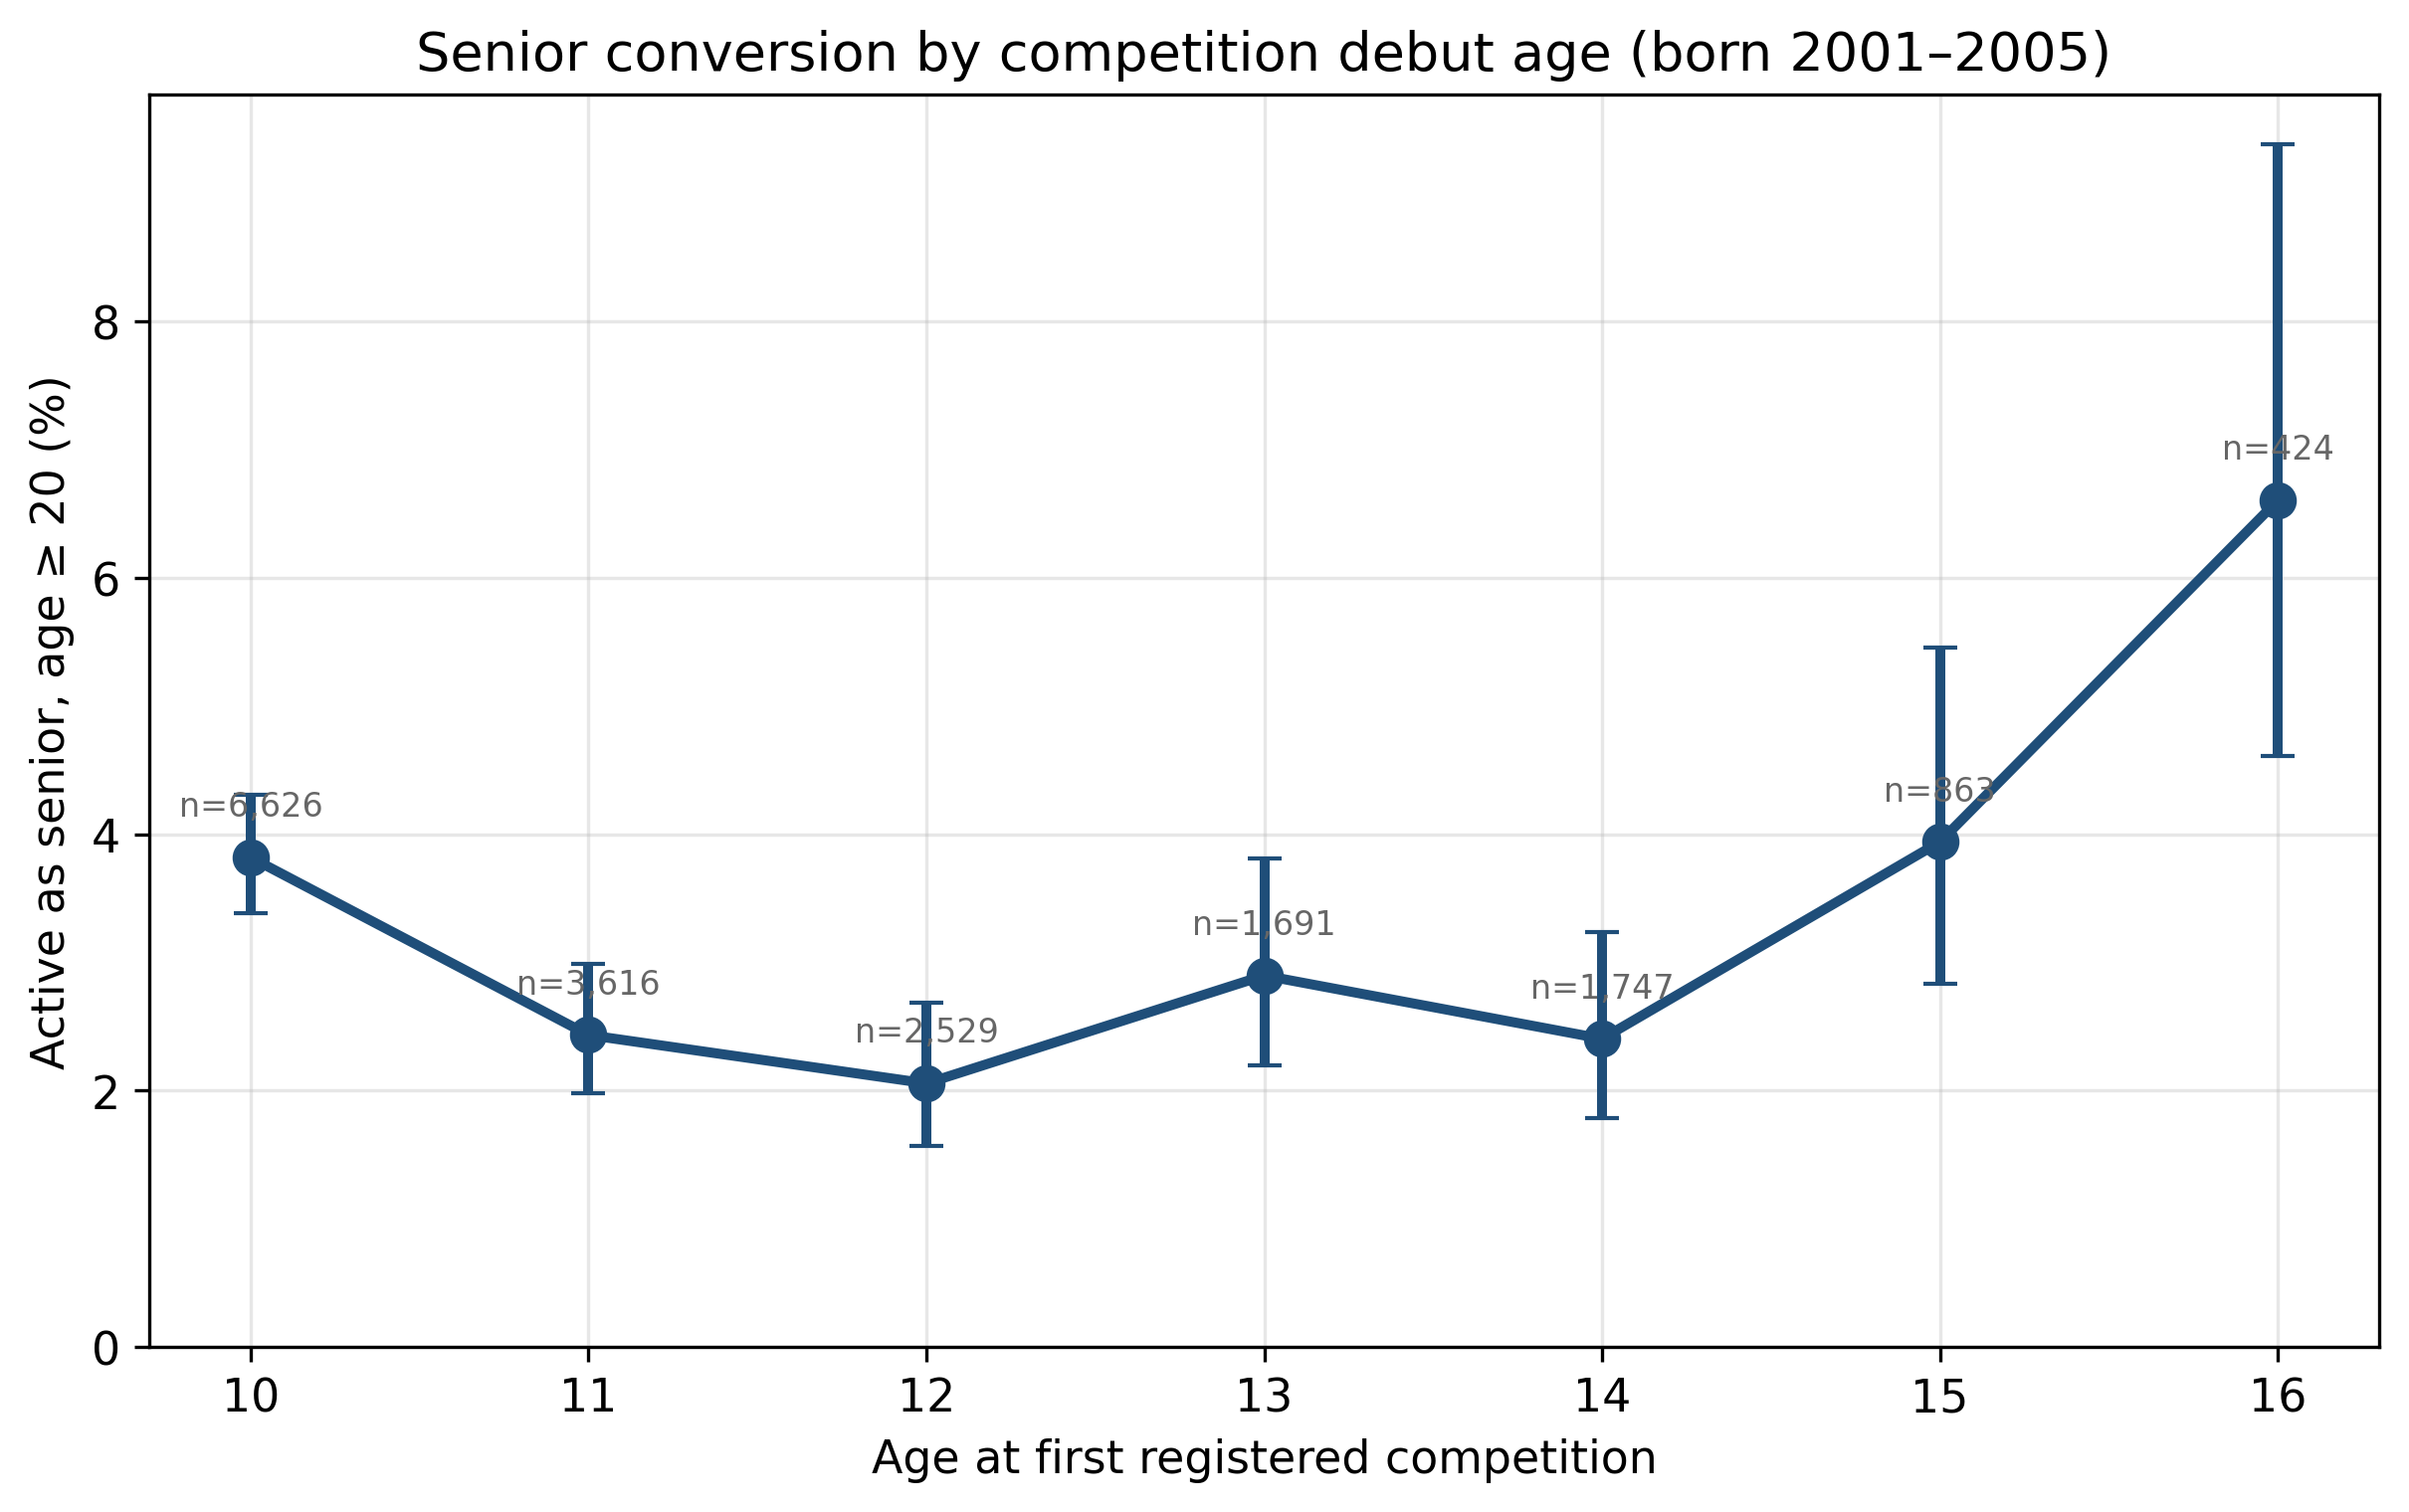
\includegraphics[width=0.85\textwidth]{fig2_senior_by_debut_age.png}
\caption{Senior conversion by competition debut age, with Wilson 95\,\% confidence intervals (born 2001--2005).}
\label{fig:ushape}
\end{figure}

\subsection{Later starters leave faster --- on their own clock (H2)}

Aligned on time since debut (Figure~\ref{fig:retk}), early entrants were far more durable. One year after the debut season, 51\,\% of those who debuted at 10 were still competing, against 34--40\,\% of those who debuted at 11--14, 26\,\% at 15, and 35\,\% at 16. Five years after debut the relative gap had widened: 17\,\% (debut 10) and 10\,\% (debut 11) were still competing, against 3--7\,\% (debuts 12--16). Denominators are fully observable athlete-years and shrink only for debut at 16 (424 at $k$ = 1 to 389 at $k$ = 5); Wilson intervals for every cell are given in Supplementary Table S3. The equal-career-length outcome gives the same picture in one model (Table~\ref{tab:h1}): 20.4\,\% of those who debuted at 10 competed on at least two days in a season four or more years later, against 12.4\,\% at 11, 8.5--8.7\,\% at 12--13 and 4.5--6.6\,\% at 14--16, an adjusted OR of 0.70 per year of later debut (95\,\% CI 0.68--0.72), essentially unchanged at five (0.69) and six years (0.66; Supplementary Table S4). The decline was concentrated between debut at 10 and 14 and did not continue beyond 14, so the per-year odds ratio summarises a gradient that levels off. The fixed-age senior outcome therefore combines two opposing forces: later entrants exit faster per year of career but have fewer years to cover before age 20, and the null linear trend in H1 is these forces cancelling. On the age clock (Figure~\ref{fig:age}), the late group had far more athletes still competing at 16 (31.0\,\% with a result at 16 or later, against 14.0 and 13.7\,\% in the earlier groups) --- partly by construction, since it includes the athletes who debuted at 16 --- and the groups were close from about 19: at 20, 4.2, 3.3 and 4.5\,\% of the three groups were still competing, and at 21, 3.4, 2.7 and 3.1\,\%. Early entry thus did not leave clearly more athletes competing at adult ages; early entrants' longer careers reflected their earlier start.

\begin{figure}[H]
\centering
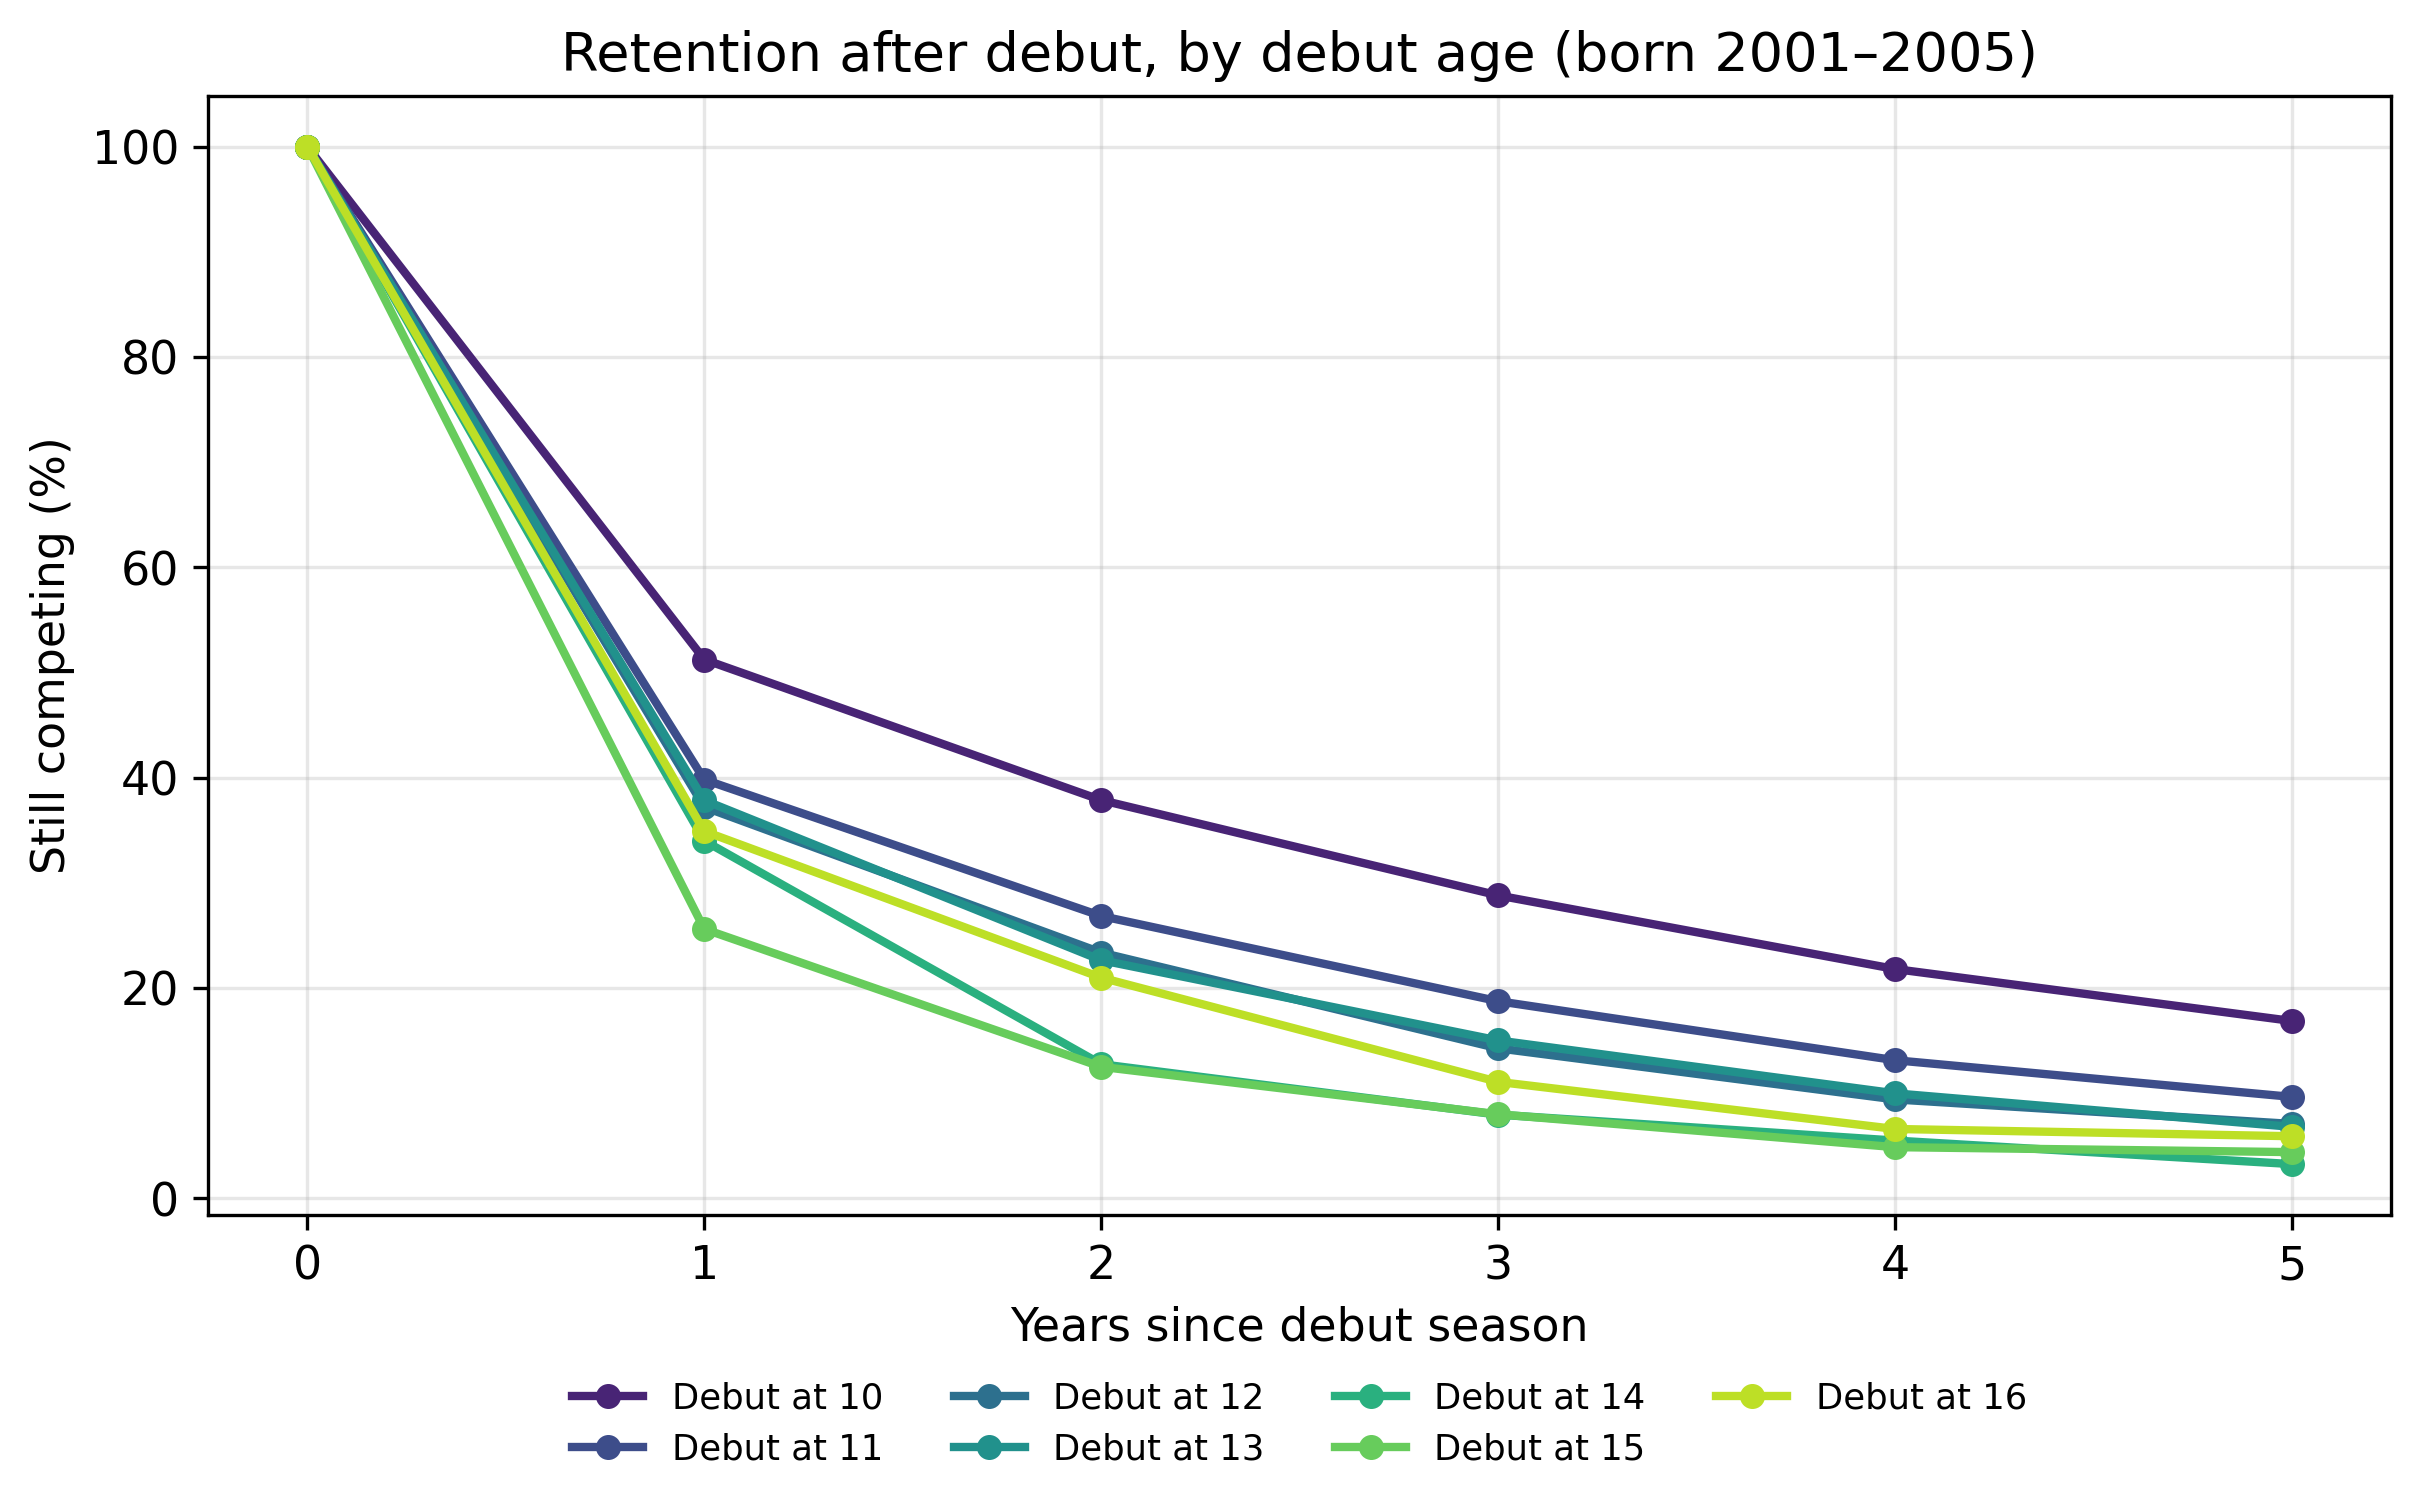
\includegraphics[width=0.85\textwidth]{fig3_retention_k.png}
\caption{Retention $k$ years after the debut season, by debut age (born 2001--2005).}
\label{fig:retk}
\end{figure}

\begin{figure}[H]
\centering
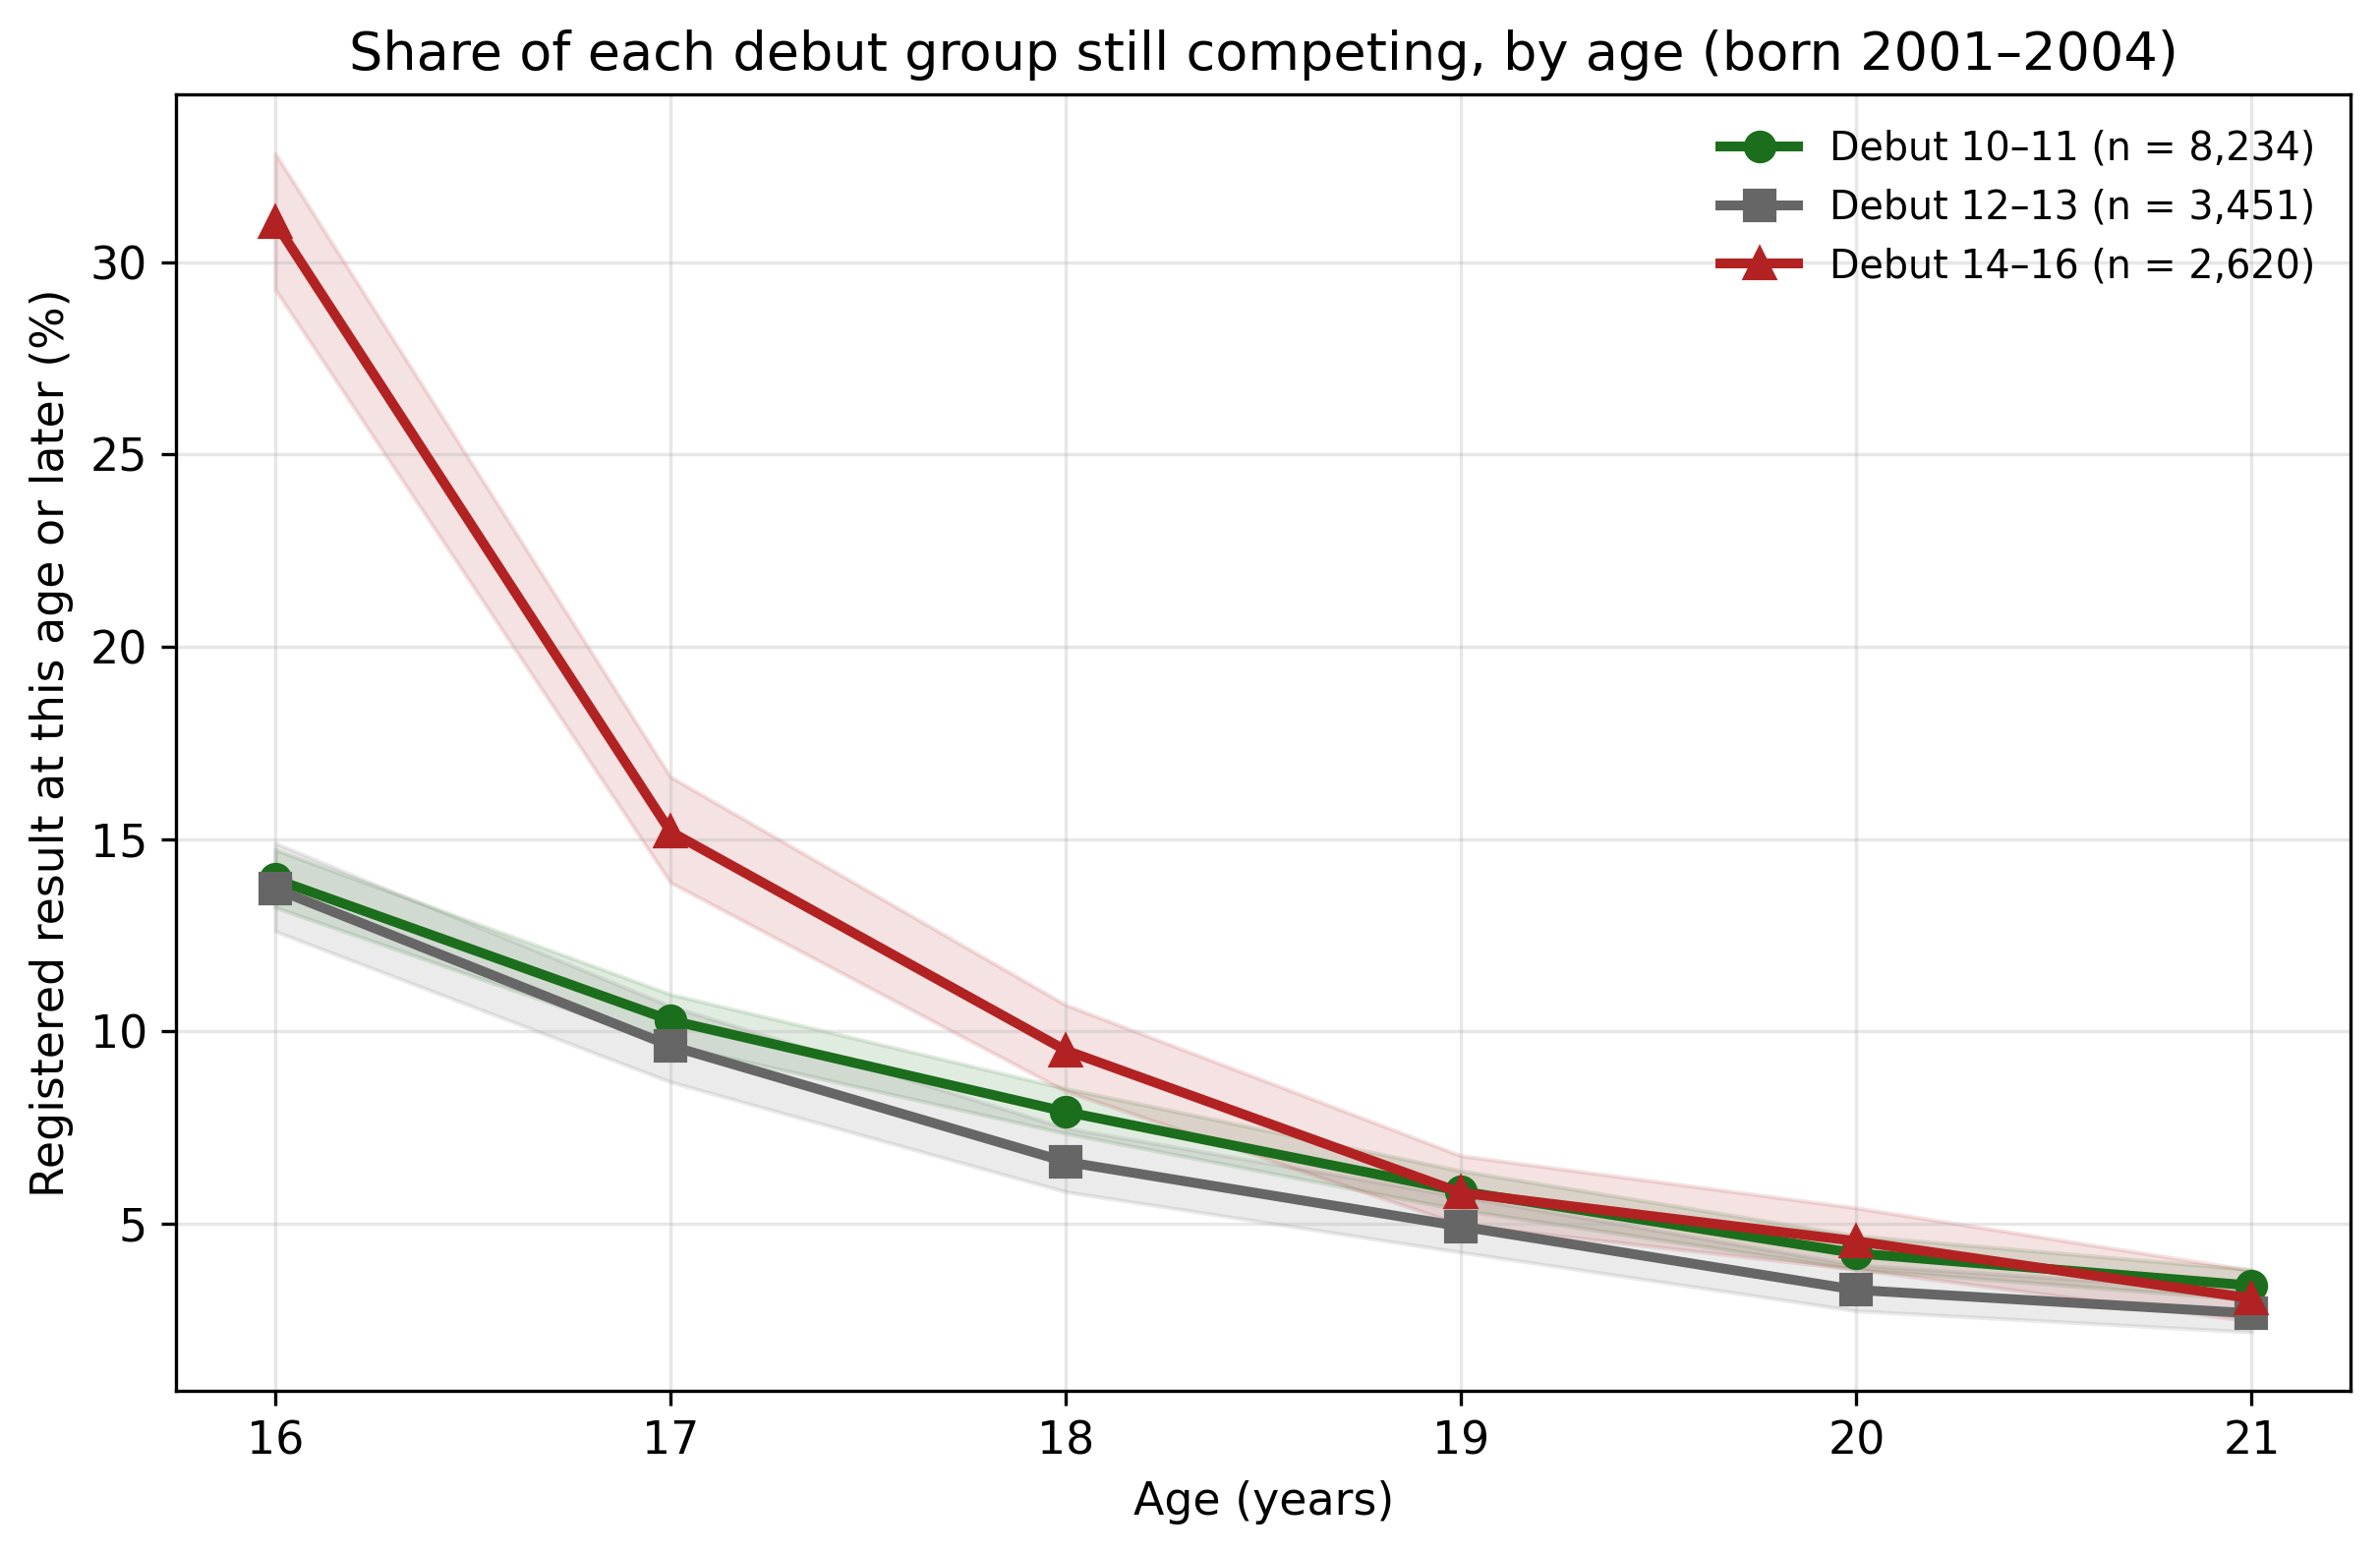
\includegraphics[width=0.85\textwidth]{fig4_shares_by_age.png}
\caption{Share of each debut group with a registered result at that age or later, cohorts born 2001--2004 (followed to age 21 for everyone), with Wilson 95\,\% confidence bands. At 16 the late group includes the athletes who debuted at that age.}
\label{fig:age}
\end{figure}

\subsection{Among survivors, entry history adds little beyond current engagement (H3)}

Of the 17\,496 debutants, 1\,637 (9.4\,\%) competed in the age-17 season itself; 472 of these (28.8\,\%) became active seniors, while 74 seniors had a fully idle age-17 season before returning --- which is exactly why the landmark must be defined on the season itself rather than on any activity at age 17 or later. In this landmark sample, earlier debut appeared advantageous: OR 0.85 per year of later debut (95\,\% CI 0.80--0.90). Adding current engagement --- competition days at ages 16--17 --- brought the association close to null (OR 0.99, 95\,\% CI 0.92--1.05). Conditional on competing at 17 and on how much the athlete competes now, when they started carries little additional predictive information. Two readings must nevertheless be kept apart: current volume is plausibly a \emph{mediator} of entry timing, and conditioning on survival to the landmark invites index-event selection, so the result licenses no claim that entry history is causally inert --- only that it adds little to prediction at the landmark. This replicates, for entry history, what earlier analyses of this registry found for early competition volume and early performance (unpublished data): in this registry, recent behaviour dominates history.

\subsection{Robustness}

None of the variations (Supplementary Table S5) moved the linear trend far from null. Excluding COVID-era debuts gave 0.95 (95\,\% CI 0.90--1.01); excluding the 2001 cohort, whose debut-at-10 season fell in the thinly covered 2011, gave 0.99; including the 549 athletes without registered sex as a separate category gave 0.99, with debut-10 conversion 3.7 instead of 3.8\,\%; the one-result senior outcome gave 1.00; activity at 17 among debuts at 10--14 gave 0.97; conditioning on debut-season volume gave a borderline 0.94 (95\,\% CI 0.89--1.00); and the cohort halves agreed on the linear trend (0.98 and 0.99) and on the non-linearity (LR test p = 7.7 $\times$ 10$^{-4}$ and 2.9 $\times$ 10$^{-5}$), but not on the elevation at 16 (OR 1.35, 95\,\% CI 0.80--2.26, for those born 2001--2003, against 3.08, 95\,\% CI 1.59--5.96, for those born 2004--2005, whose debut-16 group consists entirely of 2020--2021 debuts). Athletes debuting at 17--19 --- outside the primary range, and excluding the 165 athletes whose first registered result came at age 20 or later and could therefore coincide with the outcome itself --- converted at distinctly higher rates (OR 3.36 vs.\ debut at 10, 95\,\% CI 2.42--4.67; within the late group, 193 debuted at 17, 153 at 18 and 56 at 19), an extension of the U's right arm that is close to mechanical: a debut at 19 is a single season from the outcome window.

\FloatBarrier

% ════════════════════════════════════════════════════════════
\section{Discussion}

\subsection{Principal findings}

In the complete entry population of Norwegian youth track and field, age at first competition carried no simple message about who would still be competing as an adult. Senior conversion was U-shaped --- lowest for entrants at 11--14, back at the level of the earliest (10) entrants by 15, and highest for the latest (17--19) entrants --- with a null linear trend; the elevation at 16 rested on debuts that fell in the COVID-19 seasons. Measured from their own start, later entrants churned much faster, half of the ten-year-old debutants still competing a year after debut against roughly a quarter to a third of those debuting at 14--16, and at equal career length the share still competing fell steeply from debut at 10 to 14 and levelled off thereafter. The fixed-age U is the sum of these faster exits and the shorter distance late entrants have to the outcome age. Among athletes competing in the age-17 season, entry history added little predictive information once current competition volume was known.

\subsection{What the entry-timing margin can and cannot test}

Neither of the positions that motivated the study was formulated about this exposure, and the revision of both must respect that. The specialisation cautions concern specialised, high-volume, year-round involvement \cite{difiori2014} --- not whether a ten-year-old appears once in a sanctioned meet (the median debutant competed on a single day) --- and the statement itself describes the specialisation--burnout link as not yet demonstrated and most discontinuation as driven by time conflicts and other interests; the football finding concerns joining organised sport \cite{vanyperen2021}, whereas a ``late debutant'' here may have trained for years before a first meet. What this study tests directly is \emph{entry timing into registered competition} --- an administrable, policy-relevant variable federations actually control records for --- and it comments on the specialisation debate only indirectly. On that margin, early entry carried no retention penalty: early debutants converted better than the 11--14 entrants at the fixed age and were by far the most durable on the duration clock. The higher fixed-age conversion of those who entered at 17--19 largely reflects how close their debut lies to the outcome window, and the elevation at 16 rests largely on debuts in the COVID-19 seasons, which plausibly delayed the first registered competition of some already committed athletes; at equal career length, entrants at 14--16 persisted far less than early entrants, as the football study found for later joiners \cite{vanyperen2021}.

Beyond that mechanical distance, the two arms plausibly reflect selection, with different candidate mechanisms. On the right arm, entry at 15 and later is plausibly a decision adolescents make for themselves, and those who make it are a small, motivated, male-tilted group whose careers, when they fail, fail fast. On the left arm, several non-exclusive mechanisms could make debut at 10 beat 11--14: families with the strongest athletics attachment enrol at the first eligible age; mid-childhood entrants may be samplers arriving from other activities with weaker athletics identity; and club pathways built around training groups formed at 10 may serve later joiners less well. We present the parental-decision reading of early entry as interpretation, not evidence. And the fullest honesty is this: the entire U may be compositional --- debut age may carry no behavioural effect at all, only information about who enters when. The registry cannot see motivation, prior training, or participation in other sports, and competition debut is not the start of sport involvement.

\subsection{The first season is the universal filter}

The dominant feature of every debut group is the first-year cliff: the median debutant competed on one day, and between half and three quarters of each entry cohort did not compete in the season after debut. This parallels the registry's relative-age structure, whose selection is already complete at entry rather than produced in adolescent talent identification \cite{guttormsen2026rae}, and it extends that point from birth-date composition to participation as such: most of the selection happens at or soon after entry. Whatever determines long-term engagement, most of its action is over within a season or two of arrival, at every entry age.

\subsection{History versus current engagement, third instalment}

The landmark result extends a pattern that earlier analyses of this registry found with two other exposures (unpublished data). Early competition volume predicts senior retention, but later volume dominates it. Early performance progression predicts retention, but through the most recent window. And entry age predicts little among 17-year-old survivors once current volume is in the model. For talent systems, the registry keeps returning one lesson: \emph{as a predictor}, what an athlete is doing now outperforms any summary of how they got there. The claim is strictly predictive. Current engagement is plausibly a mediator of entry history, and the landmark conditions on survival to 17, so the attenuation of the debut coefficient is what a mediated exposure would show even if entry timing mattered causally. What follows for practice is correspondingly modest: at the landmark, entry-age heuristics add little to what current participation already says, in either direction.

\subsection{Strengths and limitations}

The strengths are completeness and design: a national registry that observes every registered debut from the first eligible age, for everyone who ever entered (not only later successes, the known weakness of retrospective expertise samples \cite{barth2022,gullich2025}), comparisons on both the age and the duration clock, a plan committed before estimation, and internal replication of the U across cohort halves (the elevation at 16 excepted). The limitations are equally structural. Competition debut is not sport start: children may train for years before their first meet, and late debutants may arrive from other sports with long athletic histories, so the exposure is entry into \emph{registered competition}. Exit from the registry is not exit from sport. Selection into debut age is unmeasured and surely strong; no causal reading is offered. Birth dates are missing for most brief early participants --- 98.5\,\% of the seniors but 51.9\,\% of the other athletes have one --- so birth-quarter shares are descriptive and no birth-quarter interaction is reported. Coverage in 2011, the first electronic season, is thinner than in later years, so some debuts at 10 in the 2001 cohort may be missing; excluding that cohort did not change H1. Registered debut also reflects registration practice --- which meets submit results for the youngest classes, and how clubs handle them --- so cohort trends in debut age (Figure~\ref{fig:cohort}) may be partly organisational rather than behavioural. Selection into debut age plausibly tracks geography, club culture, family resources, and socioeconomic access, none of which the registry measures, and the club-size proxy is defined within the study sample. Retention is not attainment: no performance data were used, so nothing here says where elite performers come from --- the retrospective expertise literature cannot speak to retention, and this study cannot speak to attainment. The senior outcome is rare (3.1\,\%), so even twofold relative differences are small in absolute terms. Finally, age equals debut age plus career duration, so no comparison separates an effect of entry age from those of age and career stage; the analysis plan's age-scale Cox model was replaced for this reason, and all H2 comparisons are descriptive.

% ════════════════════════════════════════════════════════════

% ════════════════════════════════════════════════════════════
\section{Conclusion}

In the complete entry population of Norwegian youth track and field, age at first registered competition carried no simple message about who would still be competing as an adult, and early entry carried no retention penalty: per year of career, the earliest entrants persisted longest, and no entry age from 10 to 19 failed to produce senior athletes. The decisive window was the first season or two after entry, whatever the entry age, and among athletes competing at 17, current engagement carried most of the predictive information that entry history might have offered. The latest entrants' high per-head conversion at a fixed adult age plausibly reflects their short distance to that age and self-selection rather than an advantage of entering late, so adolescents recruited into entry who would not have come on their own cannot be assumed to convert at the observed 6.6\,\% (5.4\,\% among debuts outside the COVID-19 seasons), and the late channel as observed is male-tilted. All of these statements concern participation in registered athletics, not sport participation or physical activity in general.

\section{Practical implications}

\begin{itemize}[leftmargin=*]
\item Starting competitive athletics at the earliest allowed age did not make children more likely to quit. Those who started at 10 stayed longest, year for year.
\item No age is too late to start: every entry age from 10 to 19 produced athletes who were still competing as adults.
\item Most leaving happens in the first season or two after entry, whatever the starting age. Effort to keep young athletes is better aimed at the newcomer's first seasons than at the timing of entry.
\item By late adolescence, how much an athlete currently competes says more about who stays than when they started.
\end{itemize}

\section*{Acknowledgments}

\noindent The author thanks the Norwegian Athletics Federation, whose systematic registration of competition results makes population research of this kind possible. This research did not receive any specific grant from funding agencies in the public, commercial, or not-for-profit sectors. Declarations of interest: none; the author maintains an open, non-commercial statistics platform built on the federation's public results database.

\section*{Data availability}

\noindent The competition records used in this study are publicly accessible via the Norwegian Athletics Federation's online register for ages 13 and above; records for the 10--12 age classes are not publicly released by the federation. The derived analysis dataset cannot be publicly shared because it contains personal data (athlete dates of birth) under the EU General Data Protection Regulation (GDPR). The full analysis code, with the time-stamped analysis plan, will be deposited in a public repository upon acceptance. Supplementary Tables S1--S5 accompany the submission.

\section*{Declaration of generative AI and AI-assisted technologies in the writing process}

\noindent During the preparation of this work the author used Anthropic Claude (Claude Opus 5.5) in order to improve language and readability, assist with structuring the text, check analysis code and identify errors. After using this tool, the author reviewed and edited the content as needed and takes full responsibility for the content of the publication.

\bibliographystyle{jsams}
\bibliography{references}

\end{document}
